\label {fs-acker-experiments}

We divided our evaluation of \tracker\ into three parts. Each of these parts encapsulates logically connected experiments that measure the performance of \tracker\ mechanism in various perspectives.

In Section~\ref{overhead}, we demonstrate the overhead induced by \tracker\ mechanism. First, we measure the amount of extra network traffic for different cluster sizes, the number of nodes in a logical graph, and the granularity of tracking. After that, we show throughput overhead on regular processing for a fixed streaming setup. Section~\ref{completeness} contains the evaluation of \tracker\ applied to completeness monitoring problem. We measure the notification latency within various setups as well as the ability of distributed \tracker\ to scale out. Finally, in section~\ref{snapshotting}, we figure out the performance of operator-level tracking with the state snapshotting problem. 

As a baseline approach, we utilize the marker-based method employed in Flink~\cite{Carbone:2017:SMA:3137765.3137777}. To have an ability to compare two techniques within the same streaming engine, we implemented both \tracker\ and marker methods on the top open-source distributed streaming system called \FlameStream . \FlameStream\ has similar to state-of-the-art stream processing systems (Flink, Storm, etc.) functionality and use-cases. We did not exploit any system-specific features during the implementation of tracking methods.

As a logical graph for experiments, we use simple directed graphs of various lengths. All vertices pass an input element to the next operation. All items are re-partitioned (round-robin) before each vertex. This setup does not induce possible overhead by heavy computations while covering many real-life scenarios. Graphs with few vertices (under 30) may fit almost any acyclic streaming pipeline~\cite{akidau2018streaming}. On the other hand, more massive pipelines can be considered as flattened iterative dataflows such as PageRank or Connected Components~\cite{Murray:2013:NTD:2517349.2522738, xu2016efficient}. 

We run all experiments on a cluster of 20 virtual machines with a single CPU and 4 GB RAM from one of the biggest cloud providers. Each node runs a \FlameStream\ worker. We deploy \tracker\ on nodes excluded from regular processing: a single one for centralized configuration and two for distributed configuration.

\subsection{Network usage and overhead} \label{overhead}

% https://gist.github.com/faucct/032aaf6240db361d30a184b1d7bf3c8e
\begin{figure*}[t!]
    \begin{subfigure}[b]{0.32\textwidth}
            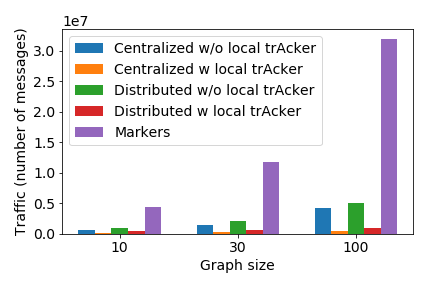
\includegraphics[width=0.99\textwidth]{pics/traffic_by_graph_size_bars.png}
            \caption{Traffic by graph size}
            \label{traffic_graph}
    \end{subfigure}
    \hspace{5mm}
    \begin{subfigure}[b]{0.32\textwidth}
            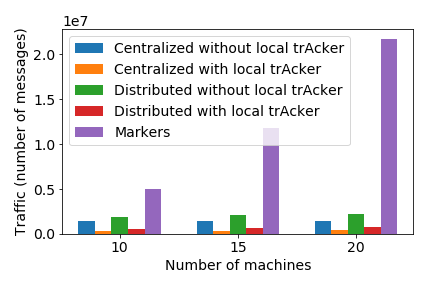
\includegraphics[width=0.99\textwidth]{pics/traffic_by_number_of_machines_bars.png}
            \caption{Traffic by number of virtual machines}
            \label{traffic_machines}
    \end{subfigure}
    \hspace{5mm}
    \begin{subfigure}[b]{0.32\textwidth}
            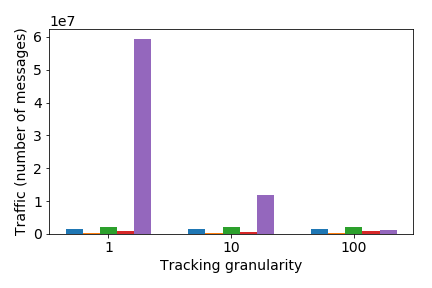
\includegraphics[width=0.99\textwidth]{pics/traffic_by_tracking_frequency_bars.png}
            \caption{Traffic by tracking frequency}
            \label{traffic_granularity}
	\end{subfigure}
    \caption{Service network traffic of marker-based approach and various \tracker\ setups}
    \label{traffic_plots}
\end{figure*}

\subsubsection{Network traffic}

We can measure the extra load provided by tracking mechanisms in a number of service messages sent over the network. In~\tracker\ there are several types of these messages: {\em Acks}, {\em Hearbeats}, {\em Min Time Updates}, and {\em Node Times} in distributed setup. In the baseline approach, all service messages are markers. Figure~\ref{traffic_plots} demonstrates the dependency between service network messages and the size of the logical graph, the number of computational nodes, and the granularity of tracking. The extra service traffic is generated by 50.000 input elements sent with 100 items per second arrival rate. 

As it is shown in Figure~\ref{traffic_graph}, service traffic for markers linearly depends on the dataflow size, because each new logical vertex adds network broadcasting of markers on a physical level. Dependency from the number of computational nodes is quadratic due to the need to broadcast markers to each node after all operators. The number of sent service messages for markers also directly depends on the tracking granularity. For example, the system should broadcast markers after each streaming element in every operator to implement tracking of individual items. 

In the case of~\tracker , service traffic depends on the logical graph size and the number of machines as well. The growth has a linear trend but can be significantly reduced with the local~\tracker\ optimization. Distributed \tracker\ without optimizations provides ~10x less service than markers traffic for a graph with 10 vertices, and ~30x decrease for a graph with 100 vertices. Regarding the number of machines, the difference is ~10x for 10 nodes, and ~30x for 20 nodes. Besides, local \tracker\ optimization allows the system to reduce traffic in up to 5 times in comparison with plain distributed \tracker .

% Network traffic was measured in number of separate service messages sent over the network. 
% Local \tracker\ was sending messages in batches.

\subsubsection{Overhead on throughput} \label{overhead}

In this experiment, we measure the median latency of regular processing, depending on the input rate (input elements per millisecond). The growth of median latency indicates the system overloading. Input rate that corresponds to the point where latency starts to growth indicates a {\em sustainable throughput}~\cite{karimov2018benchmarking}.

Figure~\ref{throughput_overhead} indicates the results of the experiment. The system without tracking at all starts to be overloaded since ~8 items per millisecond rate as well as the system with fine-grained centralized~\tracker\ setup. Overloading with the marker-based approach starts earlier and depends on the granularity of tracking: fine-grained setup does not sustain even 1 item per millisecond. Markers achieve similar to centralized~\tracker\ results only when they are injected once per 50 input elements.

This experiment shows that markers significantly bound throughput of regular processing. It is explained by the heavy extra network traffic that we demonstrated in the previous experiment. Note that this additional traffic goes through the same network channels as ordinary data items. On the other hand, \tracker\ almost does not provide additional system load due to lower extra network load and the exploiting of other network channels.

% In those experiments we compare maximum throughput of system without tracking to systems with various trackings. \tracker's overhead on maximum throughput is not substantial and does not depend on tracking window frequency. Overhead of tracking with markers is huge when tracking every element.

\begin{figure}[htbp]
  \centering
  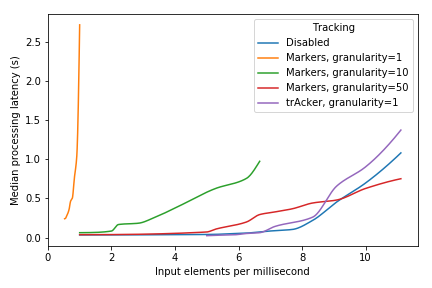
\includegraphics[width=0.50\textwidth]{pics/throughput_overhead_50.png}
  \caption{Throughput overhead}
  \label{throughput_overhead}
\end{figure}

\subsection{Completeness monitoring} \label{completeness}

\subsubsection{Notification latency}

Notification latency was measured as a time between moments of Bench Stand receiving last elements in tracking windows and notifications for that window.

% https://gist.github.com/faucct/032aaf6240db361d30a184b1d7bf3c8e
\begin{figure*}[t!]
    \begin{subfigure}[b]{0.32\textwidth}
            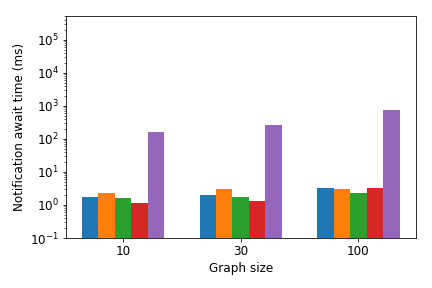
\includegraphics[width=0.99\textwidth]{pics/notification_await_time_by_graph_size_bars.png}
            \caption{Notification latency by graph size}
    \end{subfigure}
    \hspace{5mm}
    \begin{subfigure}[b]{0.32\textwidth}
            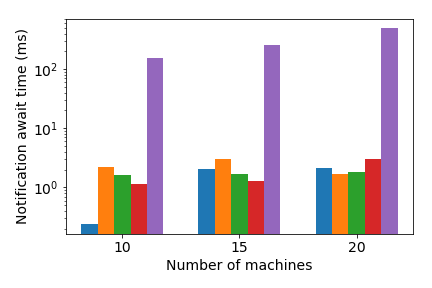
\includegraphics[width=0.99\textwidth]{pics/notification_await_time_by_number_of_machines_bars.png}
            \caption{Notification latency by number of virtual machines}
    \end{subfigure}
    \hspace{5mm}
    \begin{subfigure}[b]{0.32\textwidth}
            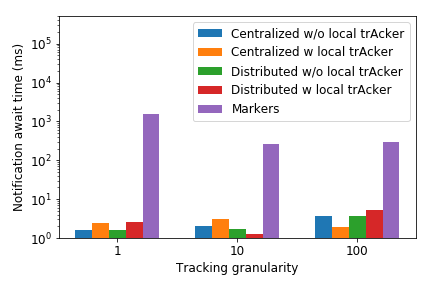
\includegraphics[width=0.99\textwidth]{pics/notification_await_time_by_tracking_frequency_bars.png}
            \caption{Notification latency by tracking frequency}
	\end{subfigure}
    \caption{Notification latency of various trackings}
\end{figure*}

\subsubsection{Scalability}

In those experiments we are reproducing a case in which the centralized \tracker\ was not holding the load, while the distributed \tracker\ was working. We have failed to reproduce it while using 100 machines running our dataflow. Still, we have been able to simulate it by increasing the total number of Ack messages.

% https://gist.github.com/faucct/546f5617b958349a125449926373b780
\begin{figure}[htbp]
  \centering
  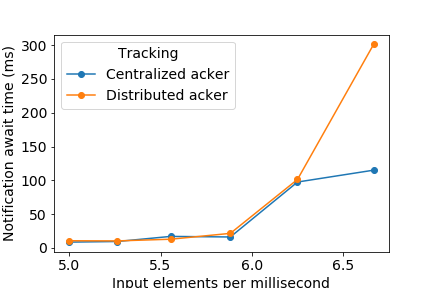
\includegraphics[width=0.50\textwidth]{pics/scalability_01x.png}
  \caption{1x acks}
\end{figure}
\begin{figure}[htbp]
  \centering
  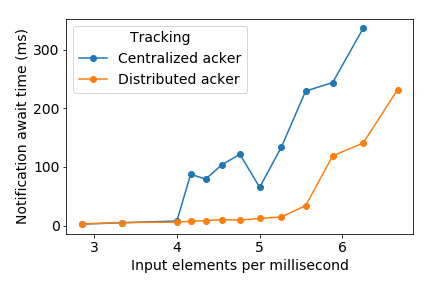
\includegraphics[width=0.50\textwidth]{pics/scalability_05x.png}
  \caption{5x acks}
\end{figure}
\begin{figure}[htbp]
  \centering
  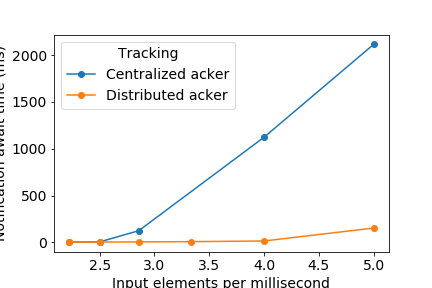
\includegraphics[width=0.50\textwidth]{pics/scalability_09x.png}
  \caption{9x acks}
\end{figure}
\begin{figure}[htbp]
  \centering
  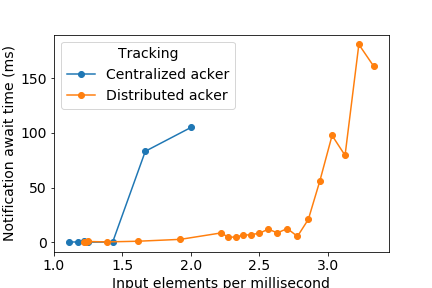
\includegraphics[width=0.50\textwidth]{pics/scalability_17x.png}
  \caption{17x acks}
\end{figure}

\subsection{State snapshotting} \label{snapshotting}

In those experiments we are comparing granular tracking using \tracker\ and markers. Processed elements are divided into snapshot windows. Pipeline vertices only process elements from a current snapshot window and buffer ones from a next snapshot window until they receive a notification that all elements from a current snapshot have been processed. When this happens vertices imitate snapshotting with a fixed duration sleep and continue to process elements from next snapshot window. We have measured a number of buffered elements and total time they have spent in buffer varying the snapshot duration.

% https://gist.github.com/faucct/6097d9d08197cb979b71721b16f8b6a3/
\begin{figure}[htbp]
  \centering
  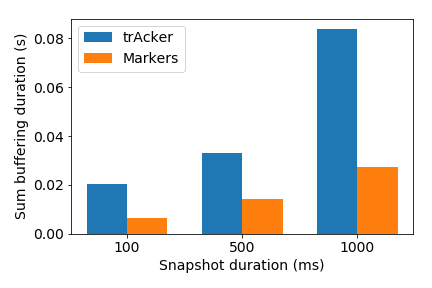
\includegraphics[width=0.50\textwidth]{pics/buffering_average_duration_bars.png}
  \caption{Average buffering duration}
\end{figure}
\begin{figure}[htbp]
  \centering
  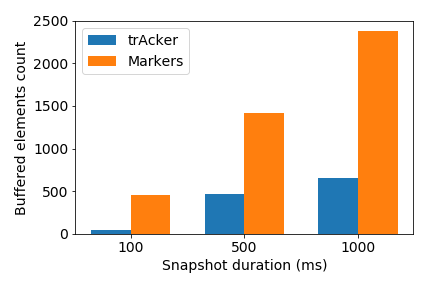
\includegraphics[width=0.50\textwidth]{pics/buffering_count_bars.png}
  \caption{Buffered elements count}
\end{figure}
\begin{figure}[htbp]
  \centering
  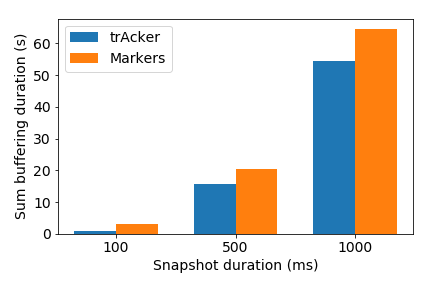
\includegraphics[width=0.50\textwidth]{pics/buffering_sum_duration_bars.png}
  \caption{Total buffering duration}
\end{figure}

\begin{figure*}[t!]
    \begin{subfigure}[b]{0.32\textwidth}
            \includegraphics[width=0.99\textwidth]{pics/buffering_latencies_barh_100.png}
            \caption{100 ms snapshot}
    \end{subfigure}
    \hspace{5mm}
    \begin{subfigure}[b]{0.32\textwidth}
            \includegraphics[width=0.99\textwidth]{pics/buffering_latencies_barh_500.png}
            \caption{500 ms snapshot}
    \end{subfigure}
    \hspace{5mm}
    \begin{subfigure}[b]{0.32\textwidth}
            \includegraphics[width=0.99\textwidth]{pics/buffering_latencies_barh_1000.png}
            \caption{1000 ms snapshot}
    \end{subfigure}
    \caption{Post-snapshot latencies}
\end{figure*}

